\documentclass[tikz,border=3pt]{standalone}
\usetikzlibrary{arrows.meta}
\begin{document}
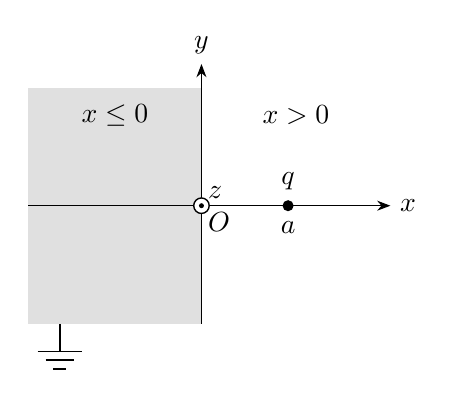
\begin{tikzpicture}[scale=1.0,>=Stealth,line width=0.9pt]
  % 導体領域 x <= 0
  \fill[black!12] (-2.2,-1.5) rectangle (0,1.5);

  % 座標軸
  \draw[line width=0.4pt,->] (-2.2,0) -- (2.4,0) node[right] {$x$};
  \draw[line width=0.4pt,->] (0,-1.5) -- (0,1.8) node[above] {$y$};

  % 原点と z 軸記号（紙面手前向き）
  \draw[line width=0.5pt,fill=white] (0,0) circle (2.8pt);
  \fill (0,0) circle (0.9pt);
  \node[above right,inner sep=2pt] at (0,0) {$z$};
  \node[below right,inner sep=2pt] at (0,0) {$O$};

  % 点電荷 q at (a, 0)
  \fill (1.1,0) circle (2.0pt);
  \node[above,yshift=2pt] at (1.1,0) {$q$};
  \node[below,yshift=-2pt] at (1.1,0) {$a$};

  % 領域ラベル（数式のみ）
  \node at (-1.1,1.15) {$x \le 0$};
  \node at (1.2,1.15) {$x > 0$};

  % 接地記号
  \draw[line width=0.6pt] (-1.8,-1.5) -- (-1.8,-1.85);
  \draw[line width=0.6pt] (-2.08,-1.85) -- (-1.52,-1.85);
  \draw[line width=0.6pt] (-1.98,-1.96) -- (-1.62,-1.96);
  \draw[line width=0.6pt] (-1.88,-2.07) -- (-1.72,-2.07);
\end{tikzpicture}
\end{document}
